\documentclass[11pt,twoside]{article}

\usepackage[nonamelimits]{amsmath}
\usepackage{amssymb, amsthm}
\usepackage{colonequals}
\usepackage{algorithm}
\usepackage{algpseudocode}

\setlength{\oddsidemargin}{0 in}
\setlength{\evensidemargin}{0 in}
\setlength{\topmargin}{-1.2 in}
\setlength{\textwidth}{6.5 in}
\setlength{\textheight}{9.5 in}
\setlength{\headheight}{0.5 in}
\setlength{\headsep}{0.5 in}
\setlength{\parindent}{0 in}
\setlength{\parskip}{0.1 in}

%%% SETS
\newcommand*{\logeq}{\ratio\Leftrightarrow}

\newcommand\Z{\mbox{$\mathbb Z$}}
\newcommand\N{\mbox{$\mathbb N$}}
\newcommand\R{\mbox{$\mathbb R$}}
\newcommand\F{\mbox{$\mathbb F$}}
\def\B{\{0,1\}}
\def\cond{\mid}

%%% FUNCTIONS
\providecommand\floor[1]{\lfloor#1\rfloor}
\providecommand\ceil[1]{\lceil#1\rceil}
\providecommand\blog[1]{\log_2\ceil{#1}}
\providecommand\abs[1]{\lvert#1\rvert}
\providecommand\bigabs[1]{\bigl\lvert#1\bigr\rvert}

\def\co{{\rm co}}
\def\avg{{\rm Avg}}
\def\heur{{\rm Heur}}

%%% THEOREM TYPE ENVIRONMENTS
\newtheorem{theorem}{Theorem}
\newtheorem{lemma}[theorem]{Lemma}
\newtheorem{corollary}[theorem]{Corollary}
\newtheorem{proposition}[theorem]{Proposition}
\newtheorem{claim}[theorem]{Claim}
\newtheorem{exercise}{Exercise}
\newtheorem{conjecture}{Conjecture}
\newtheorem{example}{Example}
\newtheorem{remark}{Remark}
\newtheorem{definition}[theorem]{Definition}

%%% HEADINGS
\newcommand{\homework}[1]{
   \pagestyle{myheadings}
   \thispagestyle{plain}
   \newpage
   \setcounter{page}{1}
   \noindent
   \classname \hfill \mbox{\updatedday} \\
   \instname \hfill \mbox{\duedate}
   \rule{6.5in}{0.5mm}
   \vspace*{-0.1 in}
}


\newcommand{\problem}[1]{\section*{Problem #1}}


\renewcommand{\labelenumi}{(\alph{enumi})}
\renewcommand{\labelenumii}{(\roman{enumii})}

%%% DEFINITIONS
\def\classname{CSCI-SHU 220: Algorithms}


%%% INSTRUCTIONS
\raggedbottom 


\usepackage[pdftex]{graphicx}
\usepackage{pgf,tikz}
\usetikzlibrary{shapes,arrows,automata}

\usepackage{listings}
\usepackage{xcolor}
\lstset { %
    language=C++,
    backgroundcolor=\color{black!5}, % set backgroundcolor
    basicstyle=\footnotesize,% basic font setting
}

\newcommand\includefa[1]{\begin{center}\includegraphics[scale=0.5]{#1}\end{center}}

\def\updatedday{Posted: February 5, 2024}
\def\duedate{Due: 11:30pm (Shanghai time), February 23, 2024}
\newenvironment{solution}{{\par\noindent\it Solution.}}{}

\def\instname{Homework 1}

\pagenumbering{gobble}

\begin{document}
\homework{1}

This assignment has in total $70$ base points and $10$ extra points, and the cap is $70$.
Bonus questions are indicated using the $\star$ mark.

\textit{Please specify the following information before submission}:
\begin{itemize}
    \item Your Name: Yufeng Xu%  (put your name here)
    \item Your NetID: yx3038% (put your NetID here)
\end{itemize}


\problem{1: Asymptotic analysis [$7+7+7$ pts]} 

\begin{enumerate}
\item Show that $n! = \omega(n^{0.99n})$.
\item Construct two functions $f,g:\mathbb{N} \rightarrow \mathbb{R}_{\geq 0}$ such that $f(n) = O(g(n))$ but neither $f(n)=o(g(n))$ nor $f(n)=\Theta(g(n))$. Show the correctness of your construction.
\item Let $f(n)=n^{0.6}$ and $g(n) = 2^{2^{\lfloor \log\log n \rfloor}}$.
Show that none of the relations $\Theta$, $O$, $\Omega$, $o$, $\omega$ applies between $f(n)$ and $g(n)$.
\end{enumerate}
\begin{solution}
\textbf{Please write down your solution to Problem 1 here.}
\vspace{0.45cm}\\
(a) want to show $n!=\omega(n^{0.99n})
\iff\forall c>0, \exists n_0>0\mid \forall n>n_0, n!>cn^{0.99n}$\\
Next, we prove it by showing $n!=\omega(n^\frac{n}{2})$\\
$n!>cn^{\frac{n}{2}}\iff\log 1+\log 2+\dots+\log n>\log c + \frac{n}{2}\log n$\\
where LHS
$=\log 1+\log 2+\dots+\log \frac{n}{2}+\log\left(\frac{n}{2}+1\right)+\dots+\log(n-1)+\log n\\
>0+\log 2+\dots+\log 2+\log 2+\log\frac{n}{4}+\log\frac{n}{2}+\dots+\log\frac{n}{2}+\log{n}\\
=\frac{n}{2}\left(\log\frac{n}{2}+\log 2\right)=\frac{n}{2}\log n$
\vspace{0.45cm}\\
(b)let $f(n)=\sin(\frac{n\pi}{2})+1, g(n)=\sin(\frac{n\pi}{2})+2$, take $b=1,
n_0=1, \forall n>n_0, f(n)\leq1\cdot g(n)$, so$f(n)=O(g(n))$\\
However, $f(n)\neq o(g(n))$ and $f(n)\neq \Theta(g(n))$
\vspace{0.3cm}\\
(i)If $f(n) = o(g(n))$, then $\forall b>0, \exists n_0>0$ such that $\forall n>n_0, f(n)<b\cdot g(n)$\\
Take $b=0.1$, assume $\exists n_0>0$ such that $\forall n>n_0, f(n)<0.1\cdot g(n)$\\
Take $n=2\ceil{n_0}>n_0, sin(\frac{2\ceil{n_0}\pi}{2})=sin(\ceil{n_0}\pi)=0$, $f(n)=0+1>0.2=0.1\cdot (0+2)=0.1\cdot g(n)$, 
contradictory to our assumption that $f(n)<c\cdot g(n)$. Therefore, $f(n)\neq o(g(n))$
\vspace{0.3cm}\\
(ii)If $f(n)=\Theta(g(n))$, then $\exists a,b>0$ such that $\exists n_0>0,\forall n>n_0,
a\cdot g(n)\leq f(n)\leq b\cdot g(n)$\\
Assume such $a,b,n_0$ exist, take $n=4\ceil{n_0}+3, sin(\frac{n\pi}{2})=sin\left((2\ceil{n_0}+\frac{3}{2})\pi\right)=-1$, therefore $f(n)=0, g(n)=1$\\
we also know $a\cdot g(n)\leq f(n)\leq b\cdot g(n)$, therefore $a=0$, 
contradictory to our essumption that $a>0$. Therefore, $f(n)\neq \Theta(g(n))$
\vspace{0.45cm}\\
(c)Consider $n=2^{2^k}, k\in \N$, then $f(n)=2^{0.6\cdot 2^k}$, $g(n)=2^{2^k}, \frac{g(n)}{f(n)}=2^{0.4\cdot 2^k}$\\
Consider $n=2^{2^k-1}, k\in \N$, then $f(n)=2^{0.6\cdot (2^k-1)}$, $g(n)=2^{2^{k-1}}, \frac{f(n)}{g(n)}=2^{0.1\cdot (2^k-6)}$
\vspace{0.3cm}\\
(i)Assume $f(n)=O(g(n)), \exists b, n_0>0$ such that $\forall n>n_0, f(n)>b\cdot g(n)$\\
However, take $k=\max\{\ceil{\log(\log n_0+1)}+1,\ceil{\log(10\cdot\log b+6)}+1\}$, take $n=2^{2^k-1}>n_0$,
then $\frac{f(n)}{g(n)}=2^{0.1\cdot(2^k-6)}>b$, which is contradictory to $f(n)\leq b\cdot g(n)$.\\
Therefore, $f(n)\neq O(g(n))$, hence $f(n)\neq \Theta(g(n)), f(n)\neq o(g(n))$.
\vspace{0.3cm}\\
(ii)Assume $f(n)=\Omega(g(n))$, $\exists a,n_0$ such that $\forall n>n_0,f(n)\geq a\cdot g(n)$.\\
Take $k=\max\{\ceil{\log\log n_0}+1,\ceil{\log(\frac{5}{2}\log \frac{1}{a})}+1\}$, take $n=2^{2^k}>n_0$, 
then $\frac{g(n)}{f(n)}=2^{0.4\cdot 2^k}>\frac{1}{a}$, which is contradictory to $f(n)\geq a\cdot g(n)$.\\
Therefore, $f(n)\neq \Omega(g(n))$, hence $f(n)\neq \omega(g(n))$. None of $\Theta, O, \Omega, o, \omega$ apply to $f(n)$ and $g(n)$.

 
\end{solution}

\problem{2: Finding the maximum/minimum [$10+10^\star$ pts]}
For an array $A$ of $n$ \textit{different} numbers (not necessarily sorted), we want to find the \textit{largest} number and the \textit{smallest} number in $A$ simultaneously.
However, we have no access to $A$.
Instead, we are given an oracle $\textsc{Compare}$ that can be used to compare the numbers in $A$.
For $i \neq j$, $\textsc{Compare}(i,j)$ returns $i$ if $A[i]>A[j]$ and returns $j$ if $A[j]>A[i]$ (recall that the numbers in $A$ are different by assumption, so we cannot have $A[i]=A[j]$ if $i \neq j$).
For convenience, let us assume $n$ is even.
\begin{enumerate}
    \item Design an algorithm which calls the $\textsc{Compare}$ oracle at most $\frac{3}{2} n - 2$ times and returns a pair $(i_\mathsf{max},i_\mathsf{min})$ such that $A[i_\mathsf{max}]$ (resp., $A[i_\mathsf{min}]$) is the largest (resp., smallest) number in $A$. Give the pseudocode and briefly justify its correctness.
    \item[(b)$^\star$] Show that any algorithm has to call the $\textsc{Compare}$ oracle $\frac{3}{2} n - 2$ times in worst case in order to find the largest and smallest numbers in $A$.
\end{enumerate}

\begin{solution}
\textbf{Please write down your solution to Problem 2 here.}\\
(a) The pseudocode is shown below:

\begin{algorithm}\label{2.1}
    \caption{pseudocode for problem 2.1}
    \begin{algorithmic}
        \State max\_idx $\gets \textsc{compare}(0,1)$
        \State min\_idx $\gets 1-$ max\_idx
        \State $i \gets 2$
        \While{$i < $ len(A)}
            \State tmp\_max $\gets \textsc{compare}(i,i+1)$
            \State tmp\_min $\gets$ $2\cdot i+1-$tmp\_max
            \State max\_idx $\gets \textsc{compare}(\text{tmp\_max,max\_idx})$
            \State min\_idx $\gets$ tmp\_min+min\_idx $-\textsc{compare}(\text{tmp\_min,min\_idx})$
            \State $i \gets i+2$
        \EndWhile\\
        \Return{(max\_idx, min\_idx)}
    \end{algorithmic}
\end{algorithm}
This algorithm compares the first two elements for 1 time. 
For every two elements in the next $n-2$ elements of the array, the algorithm compares for 3 times.
In total, the algorithm compares $1+(n-2)\cdot \frac{3}{2}=\frac{3}{2}n-2$ times.\\
Moreover, this algorithm is correct, because if we pick the larger number from every two numbers in the sequence, 
the global maximal number must be among this set. On the other hand, the global minimal number must be among the set of the smaller numbers from every two numbers.
\vspace{0.45cm}\\
(b) Let $A$ be the set of numbers that are possibly minimum but not maximum, 
$B$ be the set of numbers that are possibly maximum but not minimum,
$C$ be the set of numbers neither possibly minimum nor maximum,
$D$ be the set of numbers both possibly minimum and maximum. \\
Assume the size of the four sets are $(n_A, n_B, n_C, n_D)$.Initially, we have $(n_A, n_B, n_C, n_D)=(0, 0, 0, n)$.
The ultimate goal is $(1, 1, n-2, 0)$. With direct comparison, there are 3 types of meaningful operations(all other operations contribute to this goal less efficiently): \\
\begin{itemize}
    \item $(n_A, n_B, n_C, n_D)\rightarrow(n_A+1, n_B+1, n_C, n_D-2)$
    \item $(n_A, n_B, n_C, n_D)\rightarrow(n_A-1, n_B, n_C+1, n_D)$
    \item $(n_A, n_B, n_C, n_D)\rightarrow(n_A, n_B-1, n_C+1, n_D)$
\end{itemize}
It is not hard to see the second and the third operations must be done $n-2$ times in total, 
whereas the first operation should be done $\frac{n}{2}$ times. 
Therefore, the total number of comparisons is at least $\frac{3n}{2} - 2$.

\end{solution}

\problem{3: Solving recurrences [$4 \times 5+9$ pts]}
\begin{enumerate}
    \item Find big-$\Theta$ bounds for the following recurrences (and show your bounds are correct). For the base case, simply assume $T(n) = 1$ for all $n \leq 2$.
    \begin{enumerate}
        \item $T(n)=8T(n/3)+n^{1.5} \log^4 n + 9n$
        \item $T(n)=T(n-\sqrt{n}) + 6 \log n$
        \item $T(n)=2T(n/2)+ \frac{n}{\log n}$
        \item $T(n)= 5\sqrt{n} \cdot T(\sqrt{n}) + 2n$
    \end{enumerate}
    \item Recall the Fibonacci sequence $F_0,F_1,F_2,\dots$ defined using the recurrence $F_n = F_{n-1}+F_{n-2}$ with the base case $F_0 = 0$ and $F_1 = 1$. Prove by induction that $\phi^{n-2} \leq F_n < \phi^n$ for all $n \geq 1$, where $\phi = (1+\sqrt{5})/2$.
    Based on this, further show that $F_n = \Theta(\phi^n)$.
\end{enumerate}

\begin{solution}
\textbf{Please write down your solution to Problem 3 here.}
\vspace{0.45cm}\\
(a)(i) Let $T(n)=a\cdot T(\frac{n}{b})+f(n)$, where $a=8, b=3, f(n)=\Theta(n^{1.5}\log^4n)$\\
Because $\forall p,q>0, n^p=\omega(\log^qn), \log_3{8}>1.5$, $\exists \epsilon>0$ such that $f(n)=O(n^{log_3{8}-\epsilon})$\\
According to Master theorem, $T(n)=\Theta(n^{log_3{8}})$
\vspace{0.25cm}\\
(ii)Assume $T(n)=c\sqrt{n}\log{n}$, $T(n)-T(n-\sqrt{n})=c\left(\sqrt{n}\log(n)-\sqrt{n-\sqrt{n}}\log(n-\sqrt{n})\right)
=c\log{n}(\sqrt{n}-\sqrt{n-\sqrt{n}}\frac{\log(n-\sqrt{n})}{\log{n}})>c\log{n}(\sqrt{n}-\sqrt{n-\sqrt{n}})>c\log{n}\cdot\frac{1}{2}
(\text{because} (\sqrt{n}-\frac{1}{2})^2>n-\sqrt{n})$. Therefore $LHS>6\log{n}$ when $c\geq 12$.\\
On the other hand, $T(n)-6\log{n}-T(n-\sqrt{n})=(c\sqrt{n}-6)\log(n)-c\sqrt{n-\sqrt{n}}\log(n-\sqrt{n})$. Let $c=6$, we want to show $LHS<0
\iff(\sqrt{n}-1)\log(n)-\sqrt{n-\sqrt{n}}\log(n-\sqrt{n})<0
\iff \frac{1}{\sqrt{n}}\log(n)-\frac{1}{\sqrt{n-\sqrt{n}}}\log(n-\sqrt{n})<0$. Let $f(x)=2\frac{\log(x)}{x}, f'(x)=\frac{2}{\ln(2)}\frac{1-\ln(x)}{x^2}<0$
for $x \geq 3$. Therefore, $f(\sqrt{n})-f(\sqrt{n-\sqrt{n}})<0$ for $n>16$, hence $T(n)-T(n-\sqrt{n})<6\log{n}$ when $n>16$. Thus $T(n)=\Theta(\sqrt{n}\log{n})$.
\vspace{0.25cm}\\
(iii)View $T(n)$ as a recursion tree. Assume the tree has $k$ layers in total,
the $0^{th}$ layer has one node; the $1^{st}$ layer has 2 nodes plus $\frac{n}{\log{n}}$; 
the $2^{nd}$ layer has 4 nodes plus $2\cdot\frac{n}{2\log{\frac{n}{2}}}=\frac{n}{\log(n)-1}\dots$
the $k^{th}$ layer has $2^k$ nodes with value 1, plus $\frac{n}{\log(n)-k}$, where $k=\log{n}$\\
Therefore, $T(n)=2^k+n\cdot\sum_{i=1}^k\frac{1}{i}$. By integral test, $\ln(k) < \sum_{i=1}^k \frac{1}{i} < \ln(k) + 1$.
Therefore, $n\cdot\sum_{i=1}^k\frac{1}{i}=\Theta(n\log{k})=\Theta(n\log\log{n})$, $2^k=n=o(n\log\log{n})$.
Therefore, $T(n)=\Theta(n\log\log{n})$.
\vspace{0.25cm}\\
(iv)View $T(n)$ as a recursion tree. Assume the tree has $k$ layers in total,
the $0^{th}$ layer has one node; the $1^{st}$ layer has $5n^{\frac{1}{2}}$ nodes plus $2n$; 
the $2^{nd}$ layer has $25n^{\frac{3}{4}}$ nodes plus $5\sqrt{n}\cdot 2\sqrt{n}=10n\dots$
the $k^{th}$ layer has $5^kn^{1-\frac{1}{2^k}}$ nodes with value 1, plus $2\cdot 5^{k-1} n$,
where $k=\log{\log{n}}$. \\
Therefore, $T(n)=5^kn^{1-\frac{1}{2^k}}+\sum_{i=1}^k{2\cdot 5^{i-1}n}=5^kn^{1-\frac{1}{2^k}}+\frac{5^k-1}{2}n$,
where $5^k=5^{\log{\log{n}}}=2^{\log{5}\cdot\log\log{n}}=(\log{n})^{\log{5}}=\Theta\left((\log{n})^{\log{5}}\right)$, hence $5^kn^{1-\frac{1}{2^k}}=O(n(\log{n})^{\log{5}}), \frac{5^k-1}{2}n=\Theta(n(\log{n})^{\log{5}})$.
Therefore, $T(n)=\Theta(n(\log{n})^{\log{5}})$. 
\vspace{0.45cm}\\
(b) (i) Check $\phi^{-2}\leq F_0 < \phi^0, \phi^{-1}\leq F_1 < \phi^1$.
\vspace{0.25cm}\\
(ii) Assume for $1, 2 \dots k$, $\phi^{k-2}\leq F_k < \phi^k$.
Then $F_{k+1}=F_k+F_{k-1}\geq \phi^{k-2}+\phi^{k-3}=\phi^{k-3} \cdot (1 + \phi)
=\phi^{k-3} \cdot (1 + \frac{\sqrt{5}+1}{2})=\phi^{k-3} \cdot \phi^2=\phi^{k-1}$\\
$F_{k+1} < \phi^{k}+\phi^{k-1}=\phi^{k-1} \cdot (1+\phi)=\phi^{k-1}\cdot \phi^{2}=\phi^{k+1}$\\
Hence $\phi^{k-1}\leq F_{k+1} < \phi^{k+1}$. By induction, $\phi^{n-2}\leq F_n < \phi^{n}$ for all $n\geq 1$.
\vspace{0.25cm}\\
(iii) Now we show that $F_n=\Theta(\phi^n)$. We know $F_n=F_{n-1}+F_{n-2}$, \\
assume $F_n-A\cdot F_{n-1}=(1-A)\cdot(F_{n-1}-A\cdot F_{n-2})$, then $1=-A\cdot (1-A)$, $A^2-A-1=0$, hence $A=\frac{1+\sqrt{5}}{2}$ or $\frac{1-\sqrt{5}}{2}$.        
Hence $F_n=C_1\cdot (\frac{1+\sqrt{5}}{2})^n+C_2\cdot (\frac{1-\sqrt{5}}{2})^n$. We know that $F_0=0, F_1=1$, hence $C_1=\frac{\sqrt{5}}{5}, C_2=-\frac{\sqrt{5}}{5}$,                   
$F_n=\frac{\sqrt{5}}{5}(\frac{1+\sqrt{5}}{2})^n-\frac{\sqrt{5}}{5}(\frac{1-\sqrt{5}}{2})^n$, where $\frac{\sqrt{5}}{5}(\frac{1+\sqrt{5}}{2})^n=\Theta(\phi^n)$,
$-\frac{\sqrt{5}}{5}(\frac{1-\sqrt{5}}{2})^n=O(\phi^n)$, hence $F_n=\Theta(\phi^n)$.
\end{solution}

\problem{4: Counting intersection points [$10$ pts]}
Consider two horizontal lines $\ell_0: y = 0$ and $\ell_1:y = 1$ in the plane.
We have $n$ distinct points $a_1,\dots,a_n$ on $\ell_0$ and $n$ distinct points $b_1,\dots,b_n$ on $\ell_1$.
Note that the points $a_1,\dots,a_n$ and $b_1,\dots,b_n$ are \textit{not} necessarily sorted by their $x$-coordinates.
Now for each $i \in \{1,\dots,n\}$, we draw a segment $s_i$ connecting $a_i$ and $b_i$.
See the figure below for an example of $n = 4$.
These segments $s_1,\dots,s_n$ may intersect with each other, and for simplicity we assume no three segments intersect at the same point.
Our goal is to count the number of intersection points of $s_1,\dots,s_n$.
Formally, design an algorithm $\textsc{CountInt}(n,A,B)$ where $A[1 \dots n]$ stores the $x$-coordinates of $a_1,\dots,a_n$ and $B[1 \dots n]$ stores the $x$-coordinates of $b_1,\dots,b_n$.
The algorithm should return the number of intersection points of the segments $s_1,\dots,s_n$, and should have time complexity $O(n \log n)$.
Describe the basic idea and give the pseudocode.
Then justify its correctness and show it runs in $O(n \log n)$ time.

\begin{center}
    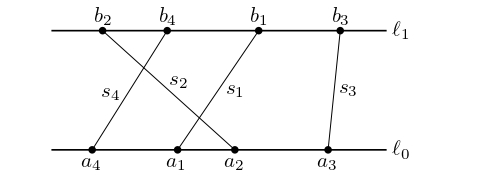
\includegraphics[height=4cm]{hw-fig-intersection.jpg}
\end{center}

\begin{solution}
\textbf{Please write down your solution to Problem 4 here.}\\
The pseudocode for this problem is shown in the next page.\\
\begin{algorithm}
    \caption{pseudocode for problem 4.1}
    \begin{algorithmic}
        \Procedure{\textsc{CountInt}}{$n,A,B$}
            \State $A\_sorted \gets \textsc{sorted}(A)$ \Comment{\textsc{sorted} is implemented by merge sort, which is $O(n\log{n})$}
            \State $B\_sorted \gets \textsc{sorted}(B)$ 
            \State $rank \gets \textsc{zeros}(n)$ \Comment{\textsc{zeros}($n$) returns an array of zeros of length $n$}
            \For{$i$ in $\textsc{range}(1, n+1)$}
                \State $rank[B\_sorted.\textsc{rank}(B[i])]=A\_sorted.\textsc{rank}(A[i])$\\
                \Comment{\textsc{rank} applies binary search($O(\log{n})$) and returns the rank of the target in a sequence.}
            \EndFor
            \Procedure{DivConq}{$m, arr$}
                \If{$m \leq 1$}
                    \State \Return $0, arr$
                \EndIf
                \State $mid \gets m/2$
                \State $m \gets \textsc{len}(arr)$
                \State $inv1, arr1 \gets$ \textsc{DivConq}($mid, arr[:mid]$)
                \State $inv2, arr2 \gets$ \textsc{DivConq}($mid, arr[mid:]$)
                \State $inv \gets inv1+inv2$
                \State $i,j \gets 1$
                \State $res \gets \textsc{emptylist}$
                \While{$i\leq\textsc{len}(arr1)$}
                    \If{$arr1[i]<arr2[j]$ OR $j>\textsc{len}(arr2)$}
                        \State $res.\textsc{append}(arr1[i])$
                        \State $i \gets i+1$
                        \State $inv \gets inv+j-1$
                    \Else
                        \State $res.\textsc{append}(arr2[j])$
                        \State $j \gets j+1$
                    \EndIf
                \EndWhile
                \State \Return $inv, arr$
            \EndProcedure
            \State $cnt, arr \gets \textsc{DivConq}(n, rank)$
            \State \Return $cnt$
        \EndProcedure     
    \end{algorithmic}
\end{algorithm}\\
This algorithm applies merge sort 2 times and binary search $2n$ times, which is $O(n\log{n})$.
In \textsc{DivConq}, the sorting of $arr1$ and $arr2$, two sorted arrays, is $O(n)$. 
In total, the time complexity of \textsc{DivConq} is $O(n\log{n})$. 
Therefore, the time complexity of the whole algorithm is $O(n\log{n})$.
Next, we will show the correctness of this algorithm.\\
We know if $a_i<a_j, b_i>b_j$, then there's an intersection between $a_i b_i$ and $a_j b_j$. 
In other words, the task of counting intersection is equivalent to counting inversed pairs.
\# inversed pairs in a sequence is equivalent to \# inversed pairs within its left part and right part,
plus \# inversed pairs across the two parts, i.e., for each entry $x$ in the left part, 
how many entries in the right part are smaller than $x$. 
By sorting $arr1$ and $arr2$, this algorithm keeps the returned array sorted and counts how many inversed pairs are there across the left and the right part.

\end{solution}

\end{document}